\documentclass[12pt]{article}
\usepackage[top=1in, bottom=1in, left=.5in, right=.5in]{geometry}
\usepackage{amsmath}
\usepackage{amssymb}
\usepackage[T1]{fontenc}
\usepackage{hyperref}
\usepackage{graphicx}
\usepackage{makecell}
\usepackage{algorithm}
\usepackage{subcaption}

\pdfpagewidth 8.5in
\pdfpageheight 11.0in
\textheight = 700pt

\setlength{\parindent}{0pt}



\begin{document}


CSI 772 \\
Homework 1 \\
Bryan Adams 

\section*{Problem 1}

\subsection*{1a}

Both resulting matrices are identical. This makes since because we are only applying transformations to the data in a different order. Both IDF and word count normalization depend on the original data, therefore, the order does not matter which order you apply. See Appendix A for python code used to normalize the data.

\subsection*{1b}

Article "tmnt raph" is the closest to "tmnt mike", reference Table \ref{tmnt_mike} for distance calculations.

\begin{table}[h!]
    \centering
    \caption{Euclidean distance between given document and the document named “tmnt mike”}
    \vspace*{4mm}
    \label{tmnt_mike}
    \begin{tabular}{c|c}
        \Xhline{3\arrayrulewidth}
        Article & Euclidean distance to "tmnt mike" \\\hline
        tmnt leo & 0.0412 \\
        tmnt raph& 0.0378 \\
        tmnt don & 0.0420 \\
        real leo & 0.0489 \\
        real raph& 0.0449 \\
        real mike& 0.0475 \\
        real don & 0.0638 \\
        \Xhline{3\arrayrulewidth}
    \end{tabular}
\end{table}

\subsection*{1c}

The distance matrix is found in Table \ref{distance_matrix}. When running hierarchical agglomerative clustering, complete linkage provides the best clusters when $K=2$ because it will cluster the Teenage Mutant Ninja Turtles articles together and the artist articles together, reference Figures \ref{fig:sub1} and \ref{fig:sub2} for the dendrograms.

\begin{table}[h!]
    \centering
    \caption{Distance matrix for documents}
    \vspace*{4mm}
    \label{distance_matrix}
    \begin{tabular}{lrrrrrrrr}
        \Xhline{3\arrayrulewidth}
        & tmnt leo & tmnt raph & tmnt mike & tmnt don & real leo & real raph & real mike & real don \\\hline
        tmnt leo & 0.0000 & 0.0386 & 0.0412 & 0.0444 & 0.0425 & 0.0496 & 0.0648 & 0.0671 \\
        tmnt raph & 0.0386 & 0.0000 & 0.0378 & 0.0429 & 0.0550 & 0.0462 & 0.0668 & 0.0688 \\
        tmnt mike & 0.0412 & 0.0378 & 0.0000 & 0.0420 & 0.0489 & 0.0449 & 0.0475 & 0.0638 \\
        tmnt don & 0.0444 & 0.0429 & 0.0420 & 0.0000 & 0.0537 & 0.0504 & 0.0619 & 0.0537 \\
        real leo & 0.0425 & 0.0550 & 0.0489 & 0.0537 & 0.0000 & 0.0394 & 0.0534 & 0.0553 \\
        real raph & 0.0496 & 0.0462 & 0.0449 & 0.0504 & 0.0394 & 0.0000 & 0.0504 & 0.0544 \\
        real mike & 0.0648 & 0.0668 & 0.0475 & 0.0619 & 0.0534 & 0.0504 & 0.0000 & 0.0580 \\
        real don & 0.0671 & 0.0688 & 0.0638 & 0.0537 & 0.0553 & 0.0544 & 0.0580 & 0.0000 \\
    \Xhline{3\arrayrulewidth}
    \end{tabular}
\end{table}

\begin{figure}
    \begin{subfigure}{0.5\textwidth}
        \centering
        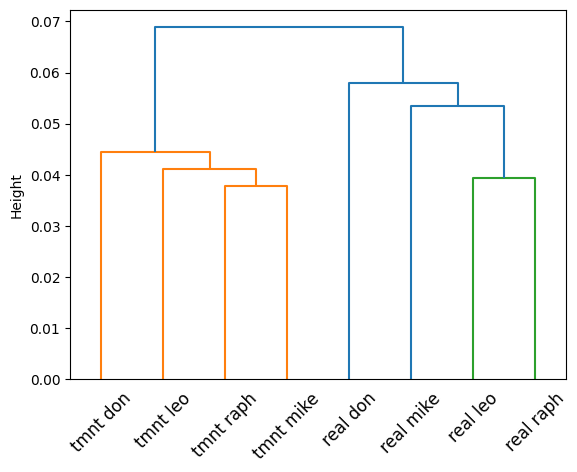
\includegraphics[width=\linewidth]{../plots/tmnt_complete.png}
        \caption{Hierarchical Agglomerative Clustering with complete linkage}
        \label{fig:sub1}
    \end{subfigure}
    \begin{subfigure}{0.5\textwidth}
        \centering
        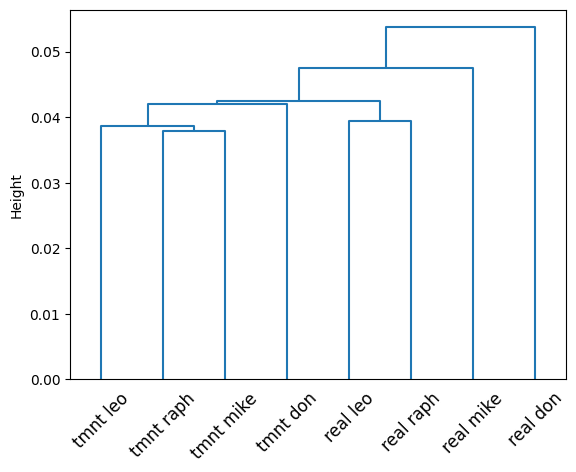
\includegraphics[width=\linewidth]{../plots/tmnt_single.png}
        \caption{Hierarchical Agglomerative Clustering with complete linkage}
        \label{fig:sub2}
    \end{subfigure}
\end{figure}


\subsection*{1d}

The top 20 most common words and their word count are found in Table \ref{word_count}. They make up 24.3425\% of the word count. It takes $\mathbf{254}$ words to account for at least 50\% of the words in the documents.

\begin{table}[h!]
    \centering
    \caption{Top 20 most common words}
    \vspace*{4mm}
    \label{word_count}
    \begin{tabular}{c|cccccccccccccccccccc}
        \Xhline{3\arrayrulewidth}
        Word & the & and & his & was & leonardo & that & for & with & michelangelo & raphael\\\hline
        Count & 2664 & 1127 & 636 & 453 & 342 & 297 & 282 & 279 & 277 & 212 \\
        \Xhline{3\arrayrulewidth}
        Word &  from & this & which & turtles & donatello & him & series & were & who & one \\\hline
        Count & 209 & 189 & 129 & 127 & 117 & 116 & 115 & 111 & 110 & 103 \\
        \Xhline{3\arrayrulewidth}
    \end{tabular}
\end{table}

\newpage

\subsection*{1e}

Our collection of 8 Wikipedia articles appears to follow Zipf's law. When looking at Figure \ref{fig:zipf}, you can see the data is generally linear with a slope = 1. This implies that the number of times words appear in our article generally follows Zipf's law.

\begin{figure}[ht!]
    \centering
    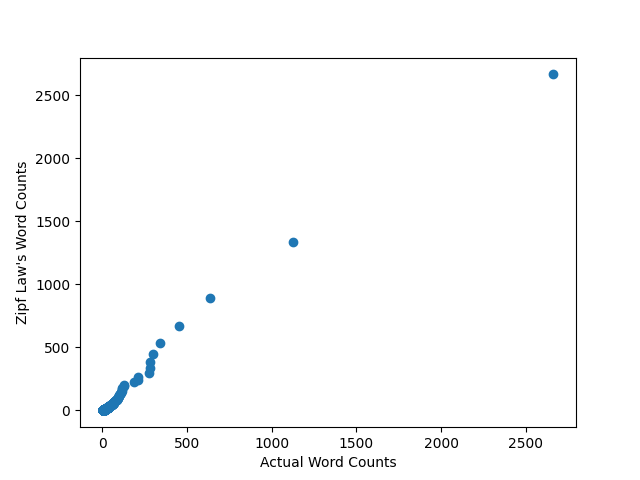
\includegraphics[width=0.5\textwidth]{../plots/zipf_law.png}
    \caption{Word counts in our articles vs Zipf's Law theoretical word counts}
    \label{fig:zipf}
\end{figure}

\clearpage


\section*{Problem 3}

\subsection*{3a,3b}

The hierarchical agglomerative clustering using both single linkage and complete linkage are found in Figure \ref{fig:3a}. Their dendrogram plots are found in Figure \ref{fig:3a_den}.

\begin{figure}[ht!]
    \begin{subfigure}{0.45\textwidth}
        \centering
        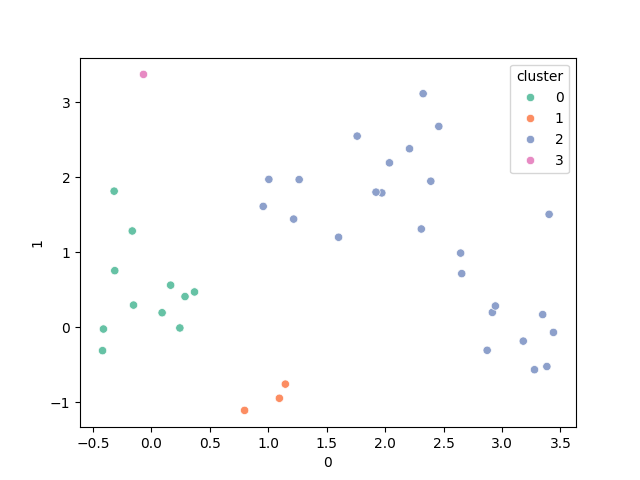
\includegraphics[width=\linewidth]{../plots/single_linkage.png}
        \caption{Problem 3 data with K=4 and using single linkage to cluster}
    \end{subfigure}
    \begin{subfigure}{0.45\textwidth}
        \centering
        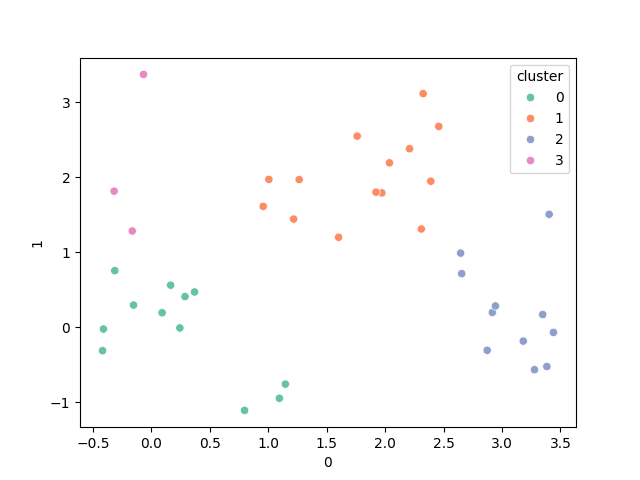
\includegraphics[width=\linewidth]{../plots/complete_linkage.png}
        \caption{Problem 3 data with K=4 and using complete linkage to cluster}
    \end{subfigure}
    \caption{Hierarchical Agglomerative Cluster plots for problems 3a and 3b}\label{fig:3a}
\end{figure}

\begin{figure}[ht!]
    \begin{subfigure}{0.45\textwidth}
        \centering
        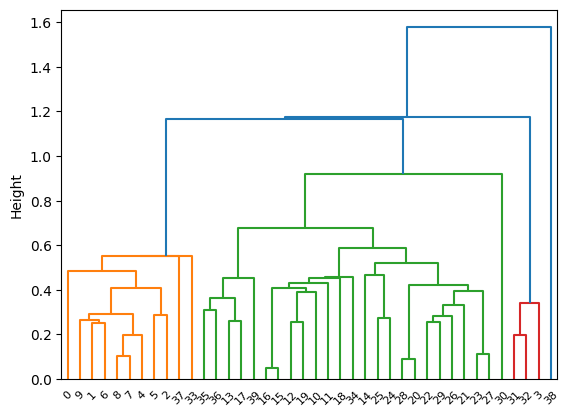
\includegraphics[width=\linewidth]{../plots/3a_single_dendrogram.png}
        \caption{Problem 3 data with K=4 and using single linkage to cluster}
    \end{subfigure}
    \begin{subfigure}{0.45\textwidth}
        \centering
        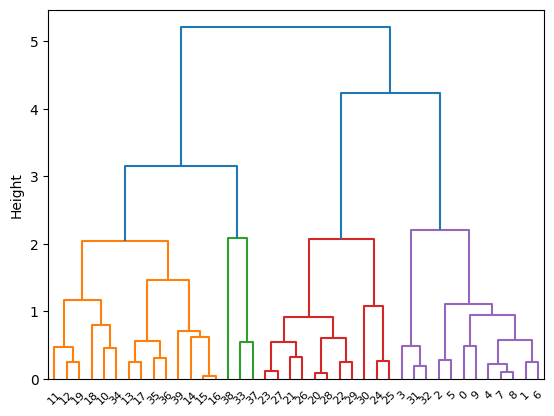
\includegraphics[width=\linewidth]{../plots/3a_complete_dendrogram.png}
        \caption{Problem 3 data with K=4 and using complete linkage to cluster}
    \end{subfigure}
    \caption{Hierarchical Agglomerative Cluster dendrogram plots for problems 3a and 3b}\label{fig:3a_den}
\end{figure}


\newpage


\subsection*{3c}
The hierarchical agglomerative clustering using both single linkage and complete linkage with the squared distances, $d_{ij}^2$ are found in Figure \ref{fig:3c}. As expected, the dendrograms did not change because $h(\cdot)$ is a monotone increase function. Their dendrogram plots are found in Figure \ref{fig:3c_den}.

\begin{figure}[ht!]
    \begin{subfigure}{0.5\textwidth}
        \centering
        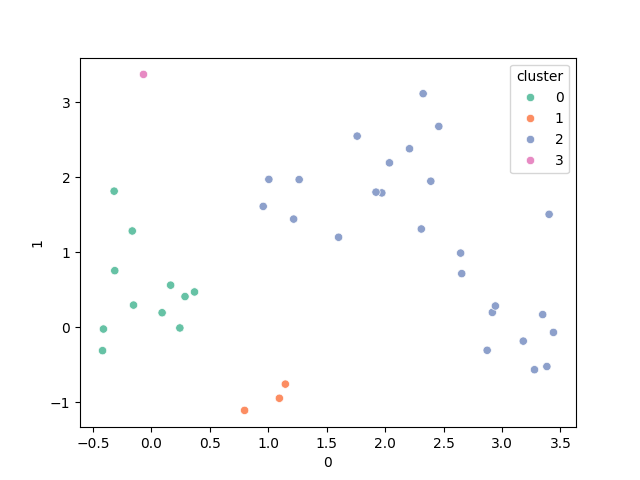
\includegraphics[width=\linewidth]{../plots/single_squared.png}
        \caption{Problem 3 data with K=4, squared distances, and using single linkage to cluster}
        \label{fig:single_squared}
    \end{subfigure}
    \begin{subfigure}{0.5\textwidth}
        \centering
        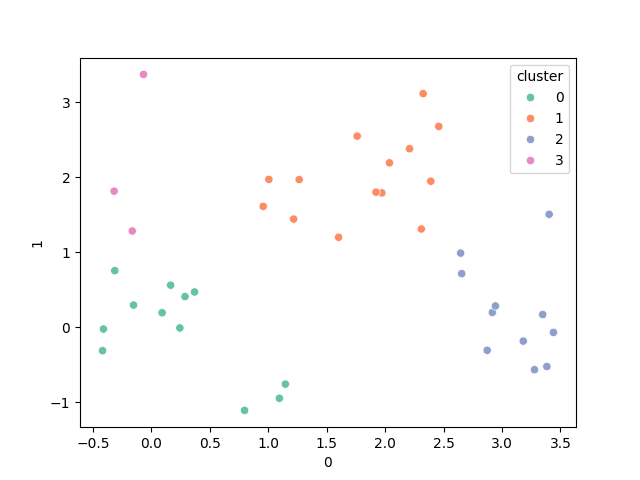
\includegraphics[width=\linewidth]{../plots/complete_squared.png}
        \caption{Problem 3 data with K=4, squared distances, and using complete linkage to cluster}
        \label{fig:complete_squared}
    \end{subfigure}
    \caption{Hierarchical Agglomerative Cluster plots for problem 3c}\label{fig:3c}
\end{figure}

\begin{figure}[ht!]
    \begin{subfigure}{0.5\textwidth}
        \centering
        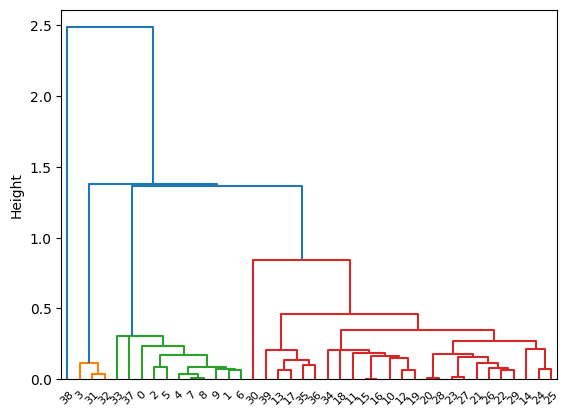
\includegraphics[width=\linewidth]{../plots/3c_single_squared_dendrogram.png}
        \caption{Problem 3 data with K=4, squared distances, and using single linkage to cluster}
    \end{subfigure}
    \begin{subfigure}{0.5\textwidth}
        \centering
        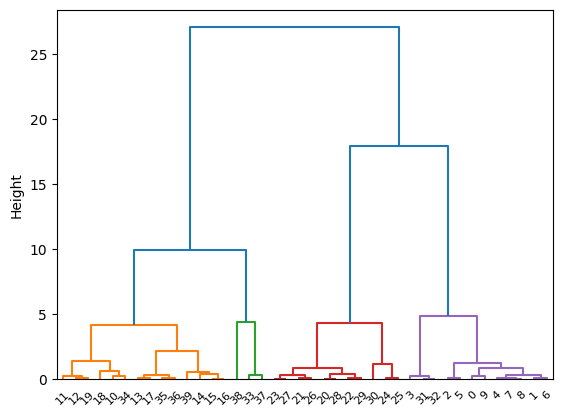
\includegraphics[width=\linewidth]{../plots/3c_complete_squared_dendrogram.png}
        \caption{Problem 3 data with K=4, squared distances, and using complete linkage to cluster}
    \end{subfigure}
    \caption{Hierarchical Agglomerative Cluster dendrogram plots for problem 3c}\label{fig:3c_den}
\end{figure}

\clearpage

\subsection*{3e}

The hierarchical agglomerative clustering using average linkage with $K=3,4$ and both $d_{ij}$ and $d_{ij}^2$ was conducted. When using $K=4$, the clusters did not change between using $d_{ij}$ and $d_{ij}^2$, reference Figures \ref{fig:average_4} and \ref{fig:average_squared_4}; however, it did change when using $K=3$, reference Figures \ref{fig:average_3} and \ref{fig:average_squared_3}. The dendrogram plots are found in Figure \ref{fig:3e_den}.

\begin{figure}[ht!]
    \begin{subfigure}{0.5\textwidth}
        \centering
        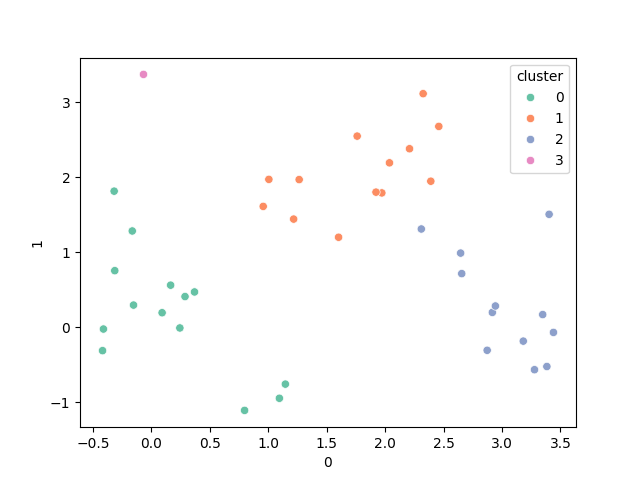
\includegraphics[width=\linewidth]{../plots/average_linkage_4.png}
        \caption{Problem 3 data with K=4, non-squared squared distances, and using average linkage to cluster}
        \label{fig:average_4}
    \end{subfigure}
    \begin{subfigure}{0.5\textwidth}
        \centering
        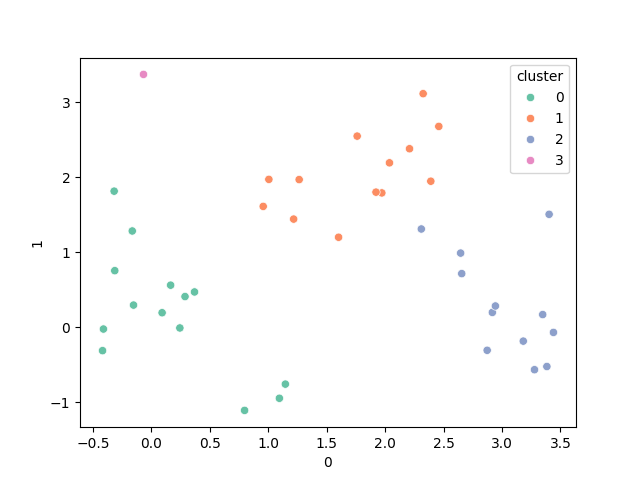
\includegraphics[width=\linewidth]{../plots/average_squared_4.png}
        \caption{Problem 3 data with K=4, squared distances, and using average linkage to cluster}
        \label{fig:average_squared_4}
    \end{subfigure}
    \begin{subfigure}{0.5\textwidth}
        \centering
        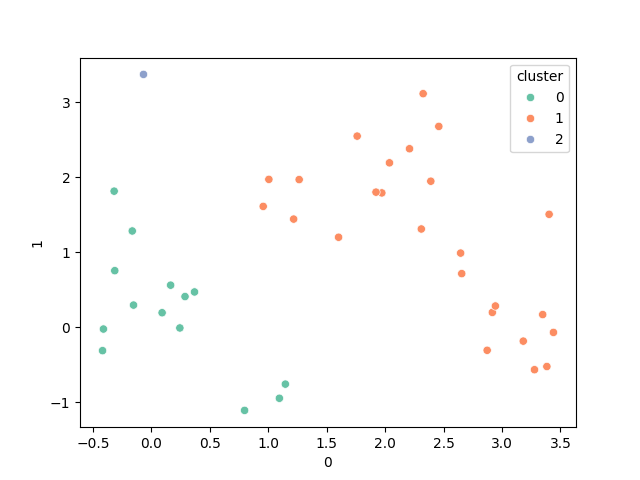
\includegraphics[width=\linewidth]{../plots/average_linkage_3.png}
        \caption{Problem 3 data with K=3, non-squared distances, and using average linkage to cluster}
        \label{fig:average_3}
    \end{subfigure}
    \begin{subfigure}{0.5\textwidth}
        \centering
        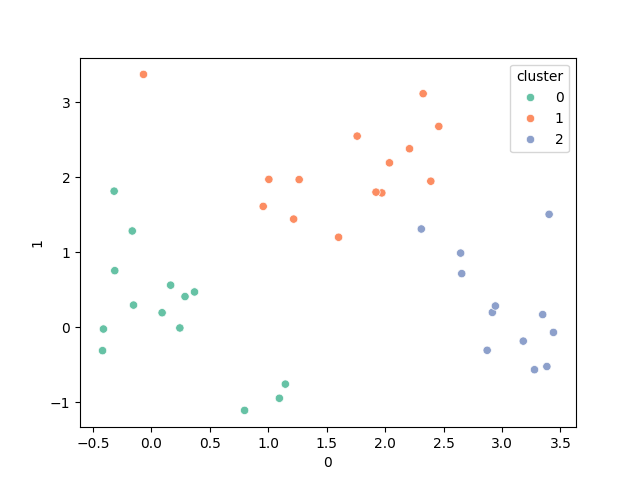
\includegraphics[width=\linewidth]{../plots/average_squared_3.png}
        \caption{Problem 3 data with K=3, squared distances, and using average linkage to cluster}
        \label{fig:average_squared_3}
    \end{subfigure}
    \caption{Hierarchical Agglomerative Cluster plots for problem 3e}
\end{figure}

\begin{figure}[ht!]
    \begin{subfigure}{0.5\textwidth}
        \centering
        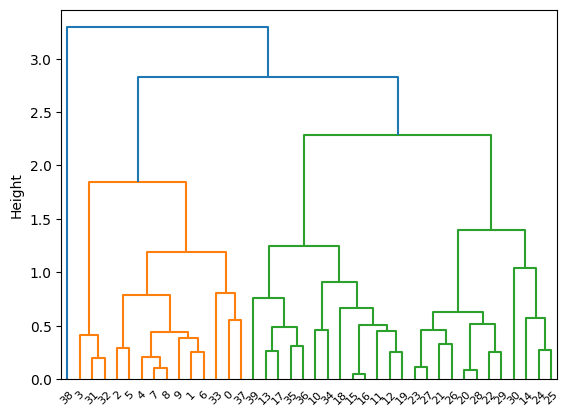
\includegraphics[width=\linewidth]{../plots/3e_average_dendrogram.png}
        \caption{Problem 3 data with K=4, squared distances, and using single linkage to cluster}
    \end{subfigure}
    \begin{subfigure}{0.5\textwidth}
        \centering
        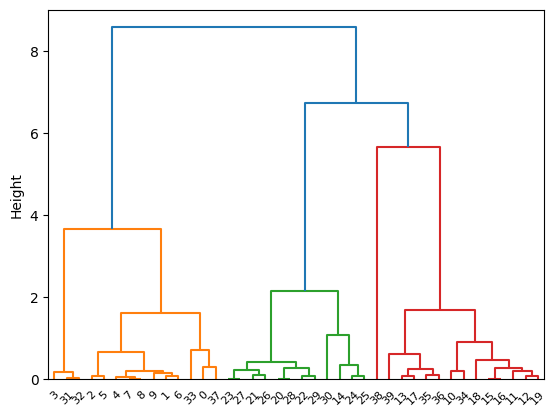
\includegraphics[width=\linewidth]{../plots/3e_average_squared_dendrogram.png}
        \caption{Problem 3 data with K=4, squared distances, and using complete linkage to cluster}
    \end{subfigure}
    \caption{Hierarchical Agglomerative Cluster dendrogram plots for problem 3c}\label{fig:3e_den}
\end{figure}

\end{document}

